\label{chapt - implementation}
Since RIL and RSSA are so similar in their structure, they share an abstract syntax tree in the implementation.
To enable variables to have indices that occur in RSSA but not in RIL, we use a tuple of type \emph{(string * int option)} as internal representation, where the string is the variable name and int option is the variable index (NONE in the RIL representation).
We alias this tuple as a \emph{var\_idx}.
Listing~\ref{listing:newName} shows the var\_idx generator used for the intermediate variables that our compiler needs.
During the second iteration of compilation we add indices to variables.
We do this by maintaining a list of tuples, which we will use for lookups to keep track of the most recently assigned index for a variable is.
It is also worth mentioning that variables in RIL and RSSA are zeroed at the beginning and end of a function. This is handled by the pretty-printer.

\lstinputlisting[label=listing:newName, caption=Here we see the var\_idx generator. It creates a new var\_idx given some input string. It uses a global counter to generate unique values for the second part of the tuple which is the int option., language=mosml] {"Listings/newName.sml"}

% Section about how to compile from the terminal
\section{Compiling from the terminal}
Compilation is done from the terminal.
Running make from the src folder create an executable \emph{hc} that can be used to compile Hermes into both C, RSSA and ARM.
When running \emph{hc} the default target language is C, but it is possible to change this with a flag such as \lstinline{--rssa} or \lstinline{--arm}.
There is a makefile in the hermes\_v4 folder which will do all of this automatically. Listing~\ref{listing:outerMakefile} shows an extract from this Makefile.
\lstinputlisting[label=listing:outerMakefile, caption=The makefile in hermes\_v4 folder has rules to compile to either RSSA or ARM., language=make, float=htp]{"Listings/outerMakefile"}

% 1: show some of the translation rules from Hermes to RIL. Also talk about the strings that are generated (inits, finits).
\section{Compilation from Hermes to RIL}
When we compile a \emph{Hermes.Update} it consists of an update-operator, an lVal that needs to be updated, an update-expression and a position.
Semantically speaking, the purpose of the \emph{Hermes.Update} is to evaluate the update-expression and update the lVal with respect to the update-operator.
% Show Hermes.Update -> RIL Assign
Listing~\ref{listing:compileStatUpdate} shows how to compile a \emph{Hermes.Update} statement: we begin by compiling the update-expression into an intermediate variable of type \lstinline{(string * int option)} that we create with our var\_idx generator. This is done in compileExp on line 3. Then we need to evaluate the lVal expression as it may contain a nested expression inside the index of an array e.g. $M[x+y]$. This is done in compileLval on line 4.
We now have some code that evaluates the update-expression as well as the lVal.
Now all we need to produce is an update which can either be an \emph{RSSA.Assign} or \emph{RSSA.MemUpdate} depending on the type of the lVal.

\lstinputlisting[label=listing:compileStatUpdate, caption=Here we see the part of the RSSA compiler that handles \emph{Hermes.Update}., language=mosml, float=tp] {"Listings/RSSACompilestatUpdate.sml"}

% 2: show some of the translation rules from RIL to RSSA. Talk about the nontrivial parts (environment, lookup function). Maybe mention invertStat and how we reverse the process. 
\section{Compilation from RIL to RSSA}
% Show RIL Assign -> RSSA Assign
Listing~\ref{listing:rssaTransformAssign} shows how an \emph{RSSA.Assign} is compiled from RIL representation to RSSA representation.
Translating RIL to RSSA requires maintaining an environment to keep track of what variables are currently in scope.
Some intermediate results from compileExp already have their indices, while Assigns with user-defined variables need to have their indices calculated.
We can leave $uop$, $r1$, $binop$ and $r2$ untouched, but we may need to update the index from RIL representation. This transformation would look something like \\
\lstinline{x := x uop r1 binop r2} \bf{->} \lstinline{x_5 := x_4 uop r1 binop r2}. \\
We first need to look up the most recent x.
This is done on line 2-3. Then we handle \lstinline{x_ii} on line 4-6 where we create a new index in case the Assign does not already have one.
On line 7 we update the environment with the new \lstinline{x_ii} and then return the updated \emph{RSSA.Assign}.
% Talk about control statements and show for loop
In case of control structures such as loop- and if-statements, most of the information needed is already given to us in \emph{Hermes.For} so we simply have to pass that along.
The body is recursively translated as shown in Listing~\ref{listing:compileStatFor}.
Converting from RIL to RSSA representation is also done recursively as shown in Listing~\ref{listing:rssaTransformFor}.
\lstinputlisting[label=listing:rssaTransformAssign, caption=Converting an \emph{RSSA.Assign} from RIL to RSSA representation is done by adding indices., language=mosml, float=tp] {"Listings/RSSATransformAssign.sml"}
\lstinputlisting[label=listing:compileStatFor, caption=\emph{Hermes.For} is handled recursively., language=mosml, float=tp] {"Listings/RSSACompilestatFor.sml"}
\lstinputlisting[label=listing:rssaTransformFor, caption=converting an \emph{RSSA.For} from RIL to RSSA representation is done by handling the body recursively., language=mosml, float=htp] {"Listings/RSSATransformFor.sml"}

% 3: show some of the translation rules from RSSA to ARM.
%       Interesting:  * abstract register names and registerallocator
%                     * side-channels and times / div (afsnit 3)
%                     * modulo implementation (hopefully not using div/mul/sub) (afsnit 3)
%                     * static array allocation
%                     * call/uncall using store and load operations as well as stack frames.
\section{Compilation from RSSA to ARM64}
For the final part of translation we need to pick what instructions we want to use for translating the different RSSA statements.
To ensure reversability we do not allow instructions such as \emph{LSL} (logical shift left) and \emph{LSR} (logical shift right) as these would throw away bits when shifting them off the end.
Instead we use \emph{ROR} (rotate right) which inserts the bits that are rotated off to the right on the vacated bit positions on the left.
We do not need to worry about only having rotate right available to us, as it can function as a rotate left if we subtract the bits we want to rotate left from $64$ and rotate right instead.
We define \emph{ROL} as a pseudo-instruction as
\begin{equation*}
  ROL(x) == ROR(64-x).
\end{equation*}
% RSSA Assign -> ARM
Listing~\ref{listing:ARMCompilestatAssign.sml} shows the compilation process for \emph{RSSA.Assign} to ARM.
Five out of six values are optional, so the amount of combinations to check for could be $1 \times 2^5 = 32$.
But not all combinations are possible, thus by pattern matching we actually reduce it to 5 different combinations:\\
The first case handles updates with constants \lstinline{xi := const c}.
The second one handles updates with array indexing \lstinline{xi := M[x]}.
The third one handles some of the intermediate results generated from the RSSA compilation step where \lstinline{xi := x}.
The fourth case handles \lstinline{xi := x uop r1}.
The fifth one handles the full \lstinline{xi := x uop r1 binop r2} that were mentioned earlier in Figure~\ref{fig:RIL vs RSSA}.

\lstinputlisting[label=listing:ARMCompilestatAssign.sml, caption=Compiling \emph{RSSA.Assign} is done by pattern matching. This reduces code size., language=mosml, float=htp] {"Listings/ARMCompilestatAssign.sml"}

\section{Logical vs physical registers}
The ARM code that is produced by our compiler uses unbounded many abstract logical registers instead of actual physical registers.
Once a register allocator is added, the code would be able to run on a device.
Register allocation requires the creation of an inteference graph, which holds information about what values are \emph{simultaneously alive}. The graph is then colored using as few colors as possible. An example is shown in Figure~\ref{fig:interferencegraph} where we see that the same register could hold values a and b as they are not alive at the same time.
In case there are too few registers/colours available to colour the interference graph, the register allocator \emph{spills} the excess values to memory by inserting store/load operations.

\begin{figure}[tp]
  \centering
  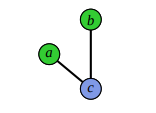
\includegraphics[scale=0.5]{Graphics/interferencegraph.png}
  \caption{An example of a coloured interference graph taken from\cite{ITU_liveness}.}
  \label{fig:interferencegraph}
\end{figure}
